\documentclass[aspectratio=169]{beamer}
\mode<presentation>
%\usetheme{Warsaw}
%\usetheme{Goettingen}
\usetheme{Hannover}
%\useoutertheme{default}

%\useoutertheme{infolines}
\useoutertheme{sidebar}
\usecolortheme{dolphin}


\setbeamersize{sidebar width left=0pt} % to remove the sidebar
\beamertemplatenavigationsymbolsempty % To remove the navigation symbols on the bottom right.
\setbeamersize{text margin left=10mm,text margin right=10mm} % Specify margins

\usepackage{amsmath}
\usepackage{amssymb}
\usepackage{listings}
\usepackage{enumerate}
\usepackage{hyperref}
\hypersetup{
    colorlinks=true,
    linkcolor=blue,
    filecolor=magenta,      
    urlcolor=cyan,
}
 
\urlstyle{same}

%some bold math symbosl
\newcommand{\Cov}{\mathrm{Cov}}
\newcommand{\Var}{\mathrm{Var}}
\newcommand{\brho}{\boldsymbol{\rho}}
\newcommand{\bSigma}{\boldsymbol{\Sigma}}
\newcommand{\btheta}{\boldsymbol{\theta}}
\newcommand{\bbeta}{\boldsymbol{\beta}}
\newcommand{\bmu}{\boldsymbol{\mu}}
\newcommand{\bW}{\mathbf{W}}
\newcommand{\one}{\mathbf{1}}
\newcommand{\bH}{\mathbf{H}}
\newcommand{\by}{\mathbf{y}}
\newcommand{\bolde}{\mathbf{e}}
\newcommand{\bx}{\mathbf{x}}

\newcommand{\cpp}[1]{\texttt{#1}}

%--------------------------------------------------
\providecommand{\abs}[1]{\lvert#1\rvert}
\providecommand{\norm}[1]{\lVert#1\rVert}
\providecommand{\Blue}[1]{\textcolor{blue}{#1}}
\providecommand{\Red}[1]{\textcolor{red}{#1}}
\newcommand{\celsius}{\ensuremath{^\circ}C}
\newcommand\thfore{\mathord{\therefore}\,}
%--------------------------------------------

\title{Lecture 14. Logical Equivalence}
%\author{BongSik Kim}
\date{ }


%\logo{\includegraphics[height=0.5cm]{Logo_PPT.pdf}}

\begin{document}
\frame[plain]{\titlepage}

\begin{frame}[plain]{The converse, contrapositive, and inverse}

 \begin{columns}[onlytextwidth]
   \begin{column}{0.6\textwidth}
     A few statements related to $p\rightarrow q$:
     \begin{itemize}
      \item The \Blue{converse} of $p\rightarrow q$ is $q\rightarrow p$.
      \item The \Blue{contrapositive} of $p\rightarrow q$ is $\neg q\rightarrow \neg p$.
      \item The \Blue{inverse} of $p\rightarrow q$ is $\neg p\rightarrow \neg q$.
     \end{itemize}

   \end{column}
  \begin{column}{0.4\textwidth}
    \centering
    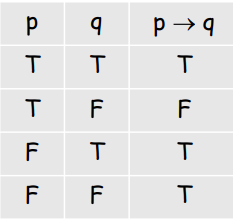
\includegraphics[height=2.7cm]{./img/lecture14-fig1.png}
  \end{column}

 \end{columns}\pause 
 
 {\bf Example 14.1.} Given the statement,
  % \begin{quote}
      \Blue{``If graph G is bipartite, it cannot contain an odd length cycle.
.}'', 
   %\end{quote}
 describe its converse, contrapositive, and inverse. \pause 
\begin{itemize}
  \item Converse: If graph G doesn't contain an odd length cycle,
       it can be bipartite. \pause
  \item Contrapositive: 
     If graph G contain an odd length cycle, it is not bipartite.\pause
  \item Inverse: If graph G is not bipartite, 
     it can contain an odd length cycle.
\end{itemize}

\pause 

   One of the three is equivalent to the original conditional statement,
WHICH ONE? How do you know?
 
\end{frame}



\begin{frame}[plain]{Logical Equivalence}


 Two statements $p$ and $q$ are  \Blue{logically equivalent}, denoted by $p\equiv q$, 
 if and only if they have the same truth values for all possible combinations of truth values 
 for the propositional variables. \pause 
 
  \begin{center}
        \begin{tabular}{|c|c|c|c|}\hline
          $p$ & $q$ & \Red{$p \rightarrow q$} &  \Blue{$q \rightarrow p$} \\ \hline
            	&   &  & \\ \hline
               &     &  &\\ \hline 
               &     &  &\\ \hline
               &     &  &\\ \hline
        \end{tabular}
        \begin{tabular}{|c|c|c|c|}\hline
          $\neg p$ & $\neg q$ & \Blue{$\neg q \rightarrow \neg p$} &  \Blue{$\neg p \rightarrow \neg q$}\\ \hline
           &   & & \\ \hline
           &  &  &\\ \hline 
           &  & &  \\ \hline
           &  &  &\\ \hline
        \end{tabular}
  \end{center} 
 \pause 
 
 \begin{itemize}
   \item The contrapositive is equivalent to the original conditional statement:
      \[ \Blue{p\rightarrow q \Leftrightarrow \neg q\rightarrow \neg p}\]
   \item The converse and inverse are equivalent to each other.
     \[ \Blue{q\rightarrow p \Leftrightarrow \neg p\rightarrow \neg q}\]
  \end{itemize}
  
\end{frame}

\begin{frame}[plain]{}

{\bf Example 14.2.} Consider the following theorem from secondary school geometry.
  \begin{quote}
     \Blue{ If a quadrilateral has a pair of parallel sides, then it has a pair of 
      supplementary angles}.~\footnote{Recall that two angles are supplementary if their angle measures sum to
      $180^\circ$}
   \end{quote}
    This theorem is of the form $p\rightarrow q$. Determine $p$ and $q$ and write the theorem 
    in its contropositive form, $\neg q\rightarrow \neg p$, which is logically equivalent to $p\rightarrow q$
 \medskip
 \pause
 
 {\bf Practice 14.3.}
 Determine if the following compound statements are logically
     equivalent.
     \begin{itemize}
       \item[(a)] $p\rightarrow q$ and $\neg p \vee q$
       \item[(b)] $\neg (p\rightarrow q)$ and $\neg p \rightarrow \neg q$
     \end{itemize}
% {\small [Send your solution to \textcolor{blue}{bkim@aurak.ac.ae}]}
\end{frame}

\begin{frame}[plain]{Propositional logic in computer programs}
 
  Statements and logical connectives arise all the time in computer programs. \pause 
  \medskip 
  
   {\bf Example 14.4.} Consider the following snippet in Python code
      \begin{center}
       
\includegraphics[height=1cm]{./img/lecture14-fig3.png}
      \end{center}
 %   \smallskip
    
 %    \hspace{.2in}   \lstinline !>> if x > 0 or (x <= 0 and y > 100):! \\
 %    \hspace{1.5in}  \lstinline !      .  !\\
 %    \hspace{1.5in}  \lstinline !      .  !\\
 %    \hspace{1.5in}  \lstinline !      .  !\\
 %     \hspace{.8in}  \lstinline !    (further instructions)  !\\
    
    \begin{itemize}
      \item The {\bf print} statement is carried out when the \emph{proposition} following the word {\bf if}
        is \emph{True}.
      \item On closer inspection, this big expression is built from two simpler propositions.\\ \pause
         \hspace{.5in} A:\ \ $x > 0$ \\
         \hspace{.5in} B:\ \  $y > 100$\pause 
      \item Then we can rewrite the 'if' condition as $\Blue{A\vee (\neg A \wedge B)}$.
      \item A truth table reveals that this complicated expression is logically equivalent to (what?).
      
    \end{itemize}


\end{frame}


\begin{frame}[plain]{ }
 \begin{itemize}
      \item (Continue from the previous example) ...  $\Blue{A\vee (\neg A \wedge B)}$.
         is logically equivalent to (what?).
         \begin{center}
        \begin{tabular}{|c|c|c|c|c|c|}\hline
          A & B & $\neg A$ & $\neg A \wedge B$ & $A\vee (\neg A \wedge B)$ &   \ \ (What?) \ \ \\ \hline
            T  &  T  &  & & & \\ \hline
            T  &  F & & & &\\ \hline 
            F	& T &  & & & \\ \hline
            F   &  F & & & & \\ \hline            
        \end{tabular}
	\end{center}\pause
     \item This means that we can simplify the code snippet without changing the program's behavior:
        \begin{center}
       
\includegraphics[height=0.9cm]{./img/lecture14-fig4.png}
      \end{center}
      \pause
    \end{itemize}
  
 
{\bf Remarks}:
  \begin{itemize}
      \item Rewriting a logical expression involving many variables in the simplest form is
        both difficult and important.
       \item Simplifying expressions in software can increase the speed of your program.
    \end{itemize}
\end{frame}

\begin{frame}[plain]{}

{\bf MSC Activity 14.5.}   
  Consider the proposition ``If AI takes over the World or outsmarts people, 
   AI will get the ability to feel emotion." 
   Write ``E" for each proposition that is logically equivalent to the given proposition,
   ``C" for each proposition that is
    logically equivalent to the converse of the given proposition and
 ``N" if neither.
 \begin{itemize} 
   \item[(a)] Unless AI gains the ability to feel an emotion, 
     AI will not dominate the world and cannot surpass humans.
   %Direct statement: If AI cannot get the ability to feel emotion, then AI cannot take over the world
   %and outsmart people.
   
   
   \item[(b)] AI does not take over the World and outsmart people, or 
        AI will get the ability to feel emotion.
   %You are younger than 21 or you can drink wine.
   
   
   \item[(c)] AI takes over the World or outsmarts people, and 
     AI will not get the ability to feel an emotion.
    %You are 21 or older and you cannot drink wine.
   
   
   \item[(d)]  AI will not get the ability to feel an emotion 
     if AI does not take over the World and outsmart people.
  % You cannot drink wine if you are younger than 21.
 
   
   \item[(e)] AI does not take over the World and outsmart people, and 
        AI will not get the ability to feel an emotion.
   %You are younger than 21 and you cannot drink wine.
\end{itemize}
 
 %ExamF22
\end{frame}
 
   

\end{document}
%--------------------------------------------------


\begin{frame}[plain]{}

  {\bf Exercise 14.1.} Determine whether the following two logic circuits are equivalent.
   
   \begin{center}
       \includegraphics[height=5cm]{lecture13-fig5.png}
      \end{center}
      
\end{frame}








    
